% -*- mode: LaTeX; -*-
%
% Copyright (C) 2011, Milan Santosi 
%
% Permission is granted to copy, distribute and/or modify this example
% under the terms of either:
%
% the GNU General Public License as published by the Free Software
% Foundation; either version 3 of the License, or (at your option) any
% later version, or
%   
% the GNU Free Documentation License, Version 1.3 or any later version
% published by the Free Software Foundation; with no Invariant Sections,
% no Front-Cover Texts, and no Back-Cover Texts.
%
% This example is distributed in the hope that it will be useful, but
% WITHOUT ANY WARRANTY; without even the implied warranty of
% MERCHANTABILITY or FITNESS FOR A PARTICULAR PURPOSE.  See the GNU
% General Public License for more details.
%
% You should have received a copy of the GNU General Public License
% and the GNU Free Document License along with this example.  If not,
% see <http://www.gnu.org/licenses/>.
%
%%%%%%%%%%%%%%%%%%%%%%%%%%%%%%%%%%%%%%%%%%%%%%%%%%%%%%%%%%%%%%%%%%%%%%%%%%%%%%%%

% This is an example of how to generate .pdf documents based on the
% style sheet of European Studies using the LateX typesetting system.
% I thought it might be something to share, so have fun with
% it. Lines that begin with % are comments.
  
% the preamble, where everything that will be required further on is loaded
\documentclass[12pt,a4paper]{article}

% needed for the TOC
\usepackage{longtable}     

% I'd prefer utf-8 but it is important to use latin1 because of
% SafeAssign. You may have to adjust the file encoding of your editor
% to iso-latin1 or iso-8859-1
\usepackage[T1]{fontenc}
\usepackage[latin1]{inputenc}

% for references with hyperlinks
\usepackage{url}

% for setting line spacing
\usepackage{setspace}

% APA-style citations and list of references thanks to Erik Meijer for
% this outstanding package!
\usepackage{apacite}

% be able to insert figures
\usepackage{graphicx}           

% these two are only needed for the title page... column layout: left
% hand side supervisor + name, right hand side your details and the
% space in between
\usepackage{multicol}
\setlength{\columnsep}{6cm}     % you may have to adjust this!

% how much additional line spacing between two footnotes?
\setlength{\footnotesep}{0cm}

% optional, as we don't use \maketitle
\author{}
\title{}
\date{}

%%%%%%%%%%%%%%%%%%%%%%%%%%%%%%%%%%%%%%%%%%%%%%%%%%%%%%%%%%%%%%%%%%%%%%%%%%%%%%%%
% the actual document begins here
\begin{document}

% line spacing 1.5 throughout (except quotations and footnotes!)
\onehalfspacing

% insert the title page at the top of our document
% Here, we define a custom title page to be inserted into the master
% document with \input{./BA2-i315648-titlepage.tex} Although the
% standard \maketitle instruction would also do the job and generates
% a nice title page too, doing it this way is recommended if you want
% your titlepage to look exactly like the European Studies style-sheet
% demands. Requires \usepackage{multicol} and
% \setlength{\columnsep}{6cm} in the preamble of the master document.

\begin{titlepage}
\begin{center}
  {
    \vspace*{5mm}    % add 0.5cm to make it about 5cm
    \Large                    % larger font for the title
    \bfseries                 % bold typeface
    
    Creating a perfect document with \LaTeX\\ and apacite.sty
  }
\end{center}
\vfill

\begin{multicols}{2}
  \normalsize
  \noindent
    Supervisor:\\*
    Kim E. Tutorsen\\*
    \\*
    \\*
    
    \noindent
    Rory Swotter\\*
    ID 0123456\\*
    Pigeonhole 737\\*
    Date: 20-04-2012\\*
    Version: final draft
    
  \end{multicols}
\end{titlepage}

\newpage

% how many levels in the ToC?
\setcounter{tocdepth}{3}

% this one keeps page numbers from being added in the footer
\pagestyle{empty}

% insert ToC and LoF with 1cm additional space in between
\tableofcontents            
\vspace{1cm} 
\listoffigures
% force another page break after the indexes
\newpage

% An opening quote
\vspace*{5mm}
\singlespacing 
\noindent
\large \textit
{
  \LaTeX is a document markup language and document preparation
  system. The term \LaTeX refers only to the language in which
  documents are written, not to the editor used to write those
  documents. In order to create a document in \LaTeX, a .tex file must
  be created using some form of text editor.
  \LaTeX is widely used in academia.
}\\*-- Wikipedia, the free encyclopedia
\normalsize
\onehalfspacing

% force a page break again and start adding page numbers to the bottom
% of each page, starting with 1
\newpage
\pagestyle{plain}
\setcounter{page}{1} 


\section{Introduction}
\label{sec:intro}
Lorem ipsum dolor sit amet\footnote{A footnote}, consectetur
adipiscing elit. Curabitur tincidunt nunc sit amet leo tincidunt eget
lobortis lacus scelerisque. Quisque varius lacinia diam ac
egestas. Pellentesque faucibus ipsum id ligula viverra nec porttitor
$x^y$ nisi pretium \cite{Tutorsen2011}. Mauris nec ligula sed nulla
dignissim cursus. Aliquam dapibus viverra erat scelerisque congue.

According to \citeA{Musterman2009}, etiam a new paragraph is indented
pharetra, purus eu auctor rutrum, justo tortor vehicula nulla, non
porta quam diam nec erat. Praesent lacinia euismod ligula, a tristique
tellus ultrices ac. Curabitur eu nisi nec purus venenatis tempus ut ac
risus. Donec eu neque convallis nunc tristique lacinia eu nec
turpis. Nam blandit dignissim sem at tempor. Ut et pellentesque
risus. Mauris semper orci sit amet mauris laoreet molestie. Nullam eu
ante tempor sem vestibulum semper. Aenean tellus purus, bibendum non
consequat a, dignissim id purus \cite[p.\ 35]{Musterman2009}. Donec
feugiat turpis nec elit scelerisque eleifend.

\newpage
\section{A Section}
\label{sec:1}

Class aptent taciti sociosqu ad litora torquent per conubia nostra,
per inceptos himenaeos. Nunc dictum fringilla metus eu commodo.  Ut
fringilla
vehicula\footnote{\url{http://www.ctan.org/what_is_tex.html}} purus,
non pulvinar diam tincidunt in. Integer convallis, lectus a mollis
semper, $x_n = \sqrt{a + b}$ felis nibh dignissim mi, quis cursus eros
est quis lorem in-text citation \cite[p.\ 19]{Abook2011}.  Proin
rhoncus blandit arcu non hendrerit. Sed mattis gravida elit, vitae
fringilla felis ultrices at. Morbi condimentum, nulla at ullamcorper
adipiscing, mauris justo mattis metus, at bibendum tellus risus id
risus.

\subsection{A subsection}
\label{sec:1-1}

Pellentesque accumsan volutpat quam quis condimentum. Proin sed metus
sem.

\begin{center}
  \begin{tabular}{ | l | l | l | p{5cm} |}
    \hline
    Day & Time & Speaker & Summary \\ \hline
    Monday & 11:00 & Socrates &  Ut scelerisque, dolor sed
    ornare tempus, ipsum lacus dapibus nibh, vel dictum sapien magna
    faucibus nibh. \\ \hline
    Tuesday & 10:00 & Wally E. Kurtz & Nulla at porttitor ante. Class aptent taciti sociosqu ad litora torquent per conubia nostra, per inceptos himenaeos. \\ \hline
    Wednesday & 18:30 & &  fiesta throughout the evening. \\
    \hline
    \end{tabular}
\end{center}

Phasellus eget mi justo, vitae tristique neque. Quisque at eleifend
ligula. Morbi quis lacinia erat. Sed sed
quam\footnote{\fullciteA{Gaudeul2006}} felis, vel ultrices
enim. Integer hendrerit est quis sapien tristique vulputate. Sed eu
ante odio, vitae euismod purus. Donec eu mollis nibh. Fusce mi nunc,
iaculis ac convallis in, varius at nibh. Duis ultricies consequat
imperdiet. Nulla facilisi. Donec semper libero sit amet metus
fermentum tincidunt.

\subsection{Another subsection}
\label{sec:1-2}

\subsubsection{A subsubsection}
\begin{figure}[h!]
\noindent 
  \centering
  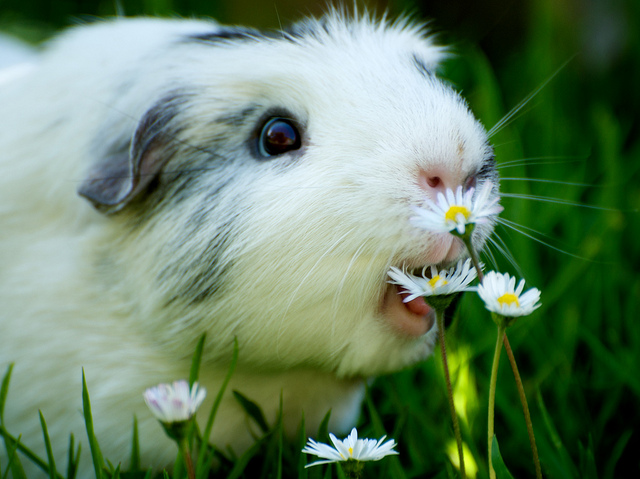
\includegraphics[width=0.5\textwidth]{omnom.jpg}
  \caption{Let's insert a picture. Source: Google images} 
\end{figure}
\noindent
Aliquam tincidunt, augue vitae rutrum sodales, eros velit gravida
nulla, sed condimentum tellus lorem sed eros. \textbf{Some bold text
  sed dolor ipsum, mollis a commodo ut, gravida ac massa}. Sed
vestibulum ultricies vehicula. Pellentesque eu ipsum congue leo
elementum hendrerit. In luctus pellentesque ipsum id viverra.Sed sed
tortor sed tortor sollicitudin accumsan. Aenean massa erat, pretium
sit amet hendrerit vel, posuere a justo.\\\\A blockquote is inserted
like this:
\singlespacing
\begin{quote}
  Nam vulputate, dui non consequat placerat, ipsum tortor fringilla
  nulla, id egestas felis elit ac mi. Phasellus eros tortor,
  sollicitudin at tincidunt vitae, ultricies ac mauris. In hac
  habitasse platea dictumst \cite[p.\ 1350]{TwoAuthors2010}
\end{quote}
\onehalfspacing
\noindent
Curabitur tortor risus, volutpat id mollis sagittis, rutrum in
quam. ``Pellentesque quotes look like this habitant morbi tristique
senectus et netus et malesuada `fames, also singlequotes' ac turpis
egestas''. Ut molestie purus quis nibh volutpat ultricies. Cras
elementum tristique blandit. Nunc vitae lectus orci, nec placerat
orci. Ut vitae turpis felis, ut fringilla nibh. \textit{Donec also
  some italic text dictum leo sit amet odio} feugiat accumsan. Morbi
euismod vulputate dolor, in consectetur lacus aliquam sed. Mauris odio
tortor, congue eu hendrerit vel, accumsan vitae purus.

\section{Another Section}
\label{sec:2}

Integer nisl nulla, pretium consequat pulvinar sed, placerat in
metus. Vivamus id turpis urna, vel sagittis ante. Cras id nulla ante,
et imperdiet odio. Nullam imperdiet molestie molestie. Nam posuere
suspendisse mattis tellus porta quam consequat ultrices adipiscing
lacus blandit. In placerat urna at ipsum sagittis volutpat. Duis
tempus dolor vitae.
\\\\
Why not have some text in columns:

\setlength{\columnsep}{1cm}
\singlespacing
\begin{multicols}{2}
\noindent  
Aenean risus lacus, feugiat quis facilisis nec, lacinia et
neque. Vestibulum ante ipsum primis in faucibus orci luctus et
ultrices posuere cubilia Curae; Nunc eu lacus ante.

Sed adipiscing, libero eu pretium varius, elit libero egestas ligula,
vitae tincidunt ante magna non diam. Nulla blandit nulla in magna
rutrum congue. Cras eu semper augue. Lorem ipsum dolor sit amet,
consectetur adipiscing elit. Fusce eu metus libero, eget aliquet
metus.
\end{multicols}
\onehalfspacing

\section{Conclusion}
\label{sec:3}
Nam sed metus sed metus cursus placerat. Duis vulputate pellentesque
ipsum, vitae cursus libero ornare eget. In congue iaculis pretium. Cum
sociis natoque penatibus et magnis dis parturient montes, nascetur
ridiculusmus \cite{Commission2002}. Suspendisse potenti. Nullam ac
cursus orci. Duis vulputate gravida est et laoreet. Donec pulvinar
tellus sem. Nam dictum tortor quis lorem pharetra sed mollis erat
pulvinar.

Class aptent taciti sociosqu ad litora torquent per conubia nostra,
per inceptos himenaeos. Aliquam dapibus placerat aliquet. 
\newpage 

%%%%%%%%%%%%%%%%%%%%%%%%%%%%%%%%%%%%%%%%%%%%%%%%%%%%%%%%%%%%%%%%%%%%%%%%%%%%%%%%
% end of document

% Insert the list of references
\bibliographystyle{apacite}
\bibliography{bibliography.bib}

% A last page
\newpage
This template was created using the following software:
\begin{itemize}
\item GNU/Emacs AUCTeX
\item \LaTeX
\item apacite.sty
\item Git scm
\end{itemize}
\vfill
Useful hyperlinks:
\begin{itemize}
\item \url{http://www.tug.org/}
\item \url{http://www.ctan.org/}
\item \url{http://en.wikibooks.org/wiki/LaTeX}
\item \url{http://www.gnu.org/software/auctex/}
\item \url{http://pdfreaders.org/}
\item \url{http://www.gnu.org/philosophy/no-word-attachments.html}
\end{itemize}

\end{document}

%%%%%%%%%%%%%%%%%%%%%%%%%%%%%%%%%%%%%%%%%%%%%%%%%%%%%%%%%%%%%%%%%%%%%%%%%%%%%%%%
% end of file

%%% Local Variables: 
%%% mode: latex
%%% TeX-master: t
%%% End: 
